\documentclass[a4paper,14pt]{extarticle}
\usepackage[left=2cm,right=2cm, top=2cm,bottom=2cm, bindingoffset=0cm]{geometry}
\usepackage[T2A]{fontenc}
\usepackage[utf8]{inputenc}
\usepackage[english,russian]{babel}
\usepackage{amsmath,amsfonts,amssymb,amsthm,mathtools,graphicx}
\usepackage{fancybox,fancyhdr}
\usepackage{tabularx}
\usepackage{multirow}
\usepackage{bigstrut}
\usepackage{booktabs}
\usepackage{float}
\usepackage{xcolor}
\usepackage{array}
\usepackage{caption}
\usepackage{url}

\DeclareGraphicsExtensions{.pdf,.png,.jpg}

\author{Ануфриев Андрей}
\title{Лабораторная работа № 3.13 \\ Магнитное поле Земли}
\date{08.05.2026}

\begin{document}

    \begin{figure}[h]
        \centering
        \begin{minipage}{0.45\linewidth}
            \centering
            
\includegraphics[width=\linewidth]{slogan_chernyy}
            \label{fig:slogan}
        \end{minipage}
        \hfill
        \begin{minipage}{0.45\linewidth}
            \centering
            
\includegraphics[width=\linewidth]{cs-logo}
            \label{fig:logo}
        \end{minipage}
    \end{figure}
    \begin{table}[htbp]
        \centering
        \small
        \begin{tabular}{@{}p{0.22\linewidth}p{0.25\linewidth}p{0.22\linewidth}p{0.20\linewidth}@{}}
            Группа & P3219 & К работе допущен & \\
            \cmidrule{2-2}\cmidrule{4-4}
            Студент & Торопов П.К. & Работа выполнена & \\
            \cmidrule{2-2}\cmidrule{4-4}
            Преподаватель & Коробков М.П. & Отчет принят & \\
            \cmidrule{2-2}\cmidrule{4-4}
        \end{tabular}%
    \end{table}%
    \vspace{2cm}
    \begin{center}
        \LARGE
        Отчет по лабораторной работе № 3.13 \\
        Магнитное поле Земли
    \end{center}
    \vspace{13cm}
    \begin{center}
        2026 год
    \end{center}
    \newpage

% ===== ЦЕЛИ =====
\section{Цели работы}
\begin{enumerate}
    \item Измерить направление суммарного магнитного поля системы катушек Гельмгольца и магнитного поля Земли.
    \item Определить горизонтальную составляющую магнитного поля Земли по зависимости $B_c(\gamma)$.
    \item Оценить качество линейной аппроксимации и сравнить экспериментальный результат с табличным значением.
\end{enumerate}

% ===== РАБОЧИЕ ФОРМУЛЫ =====
\section{Рабочие формулы и теоретические сведения}

Из методички ЛР 3.13 используются соотношения:
\begin{equation}
\frac{\sin \alpha_i}{\sin (\varphi-\alpha_i)} = \frac{B_h}{B_c},
\end{equation}
\begin{equation}
\gamma_i = \frac{\sin \alpha_i}{\sin (\varphi-\alpha_i)}, \qquad B_c = B_h\,\gamma,
\end{equation}
\begin{equation}
B_c = \mu_0\left(\frac{4}{5}\right)^{3/2}\frac{nI}{R}.
\end{equation}
Здесь $n=100$ --- число витков в каждой катушке, $R=0.15$ м --- радиус катушек, $I$ --- ток в катушках. Для построения графика и оценки $B_h$ используются рабочие точки с углами $\alpha=10^\circ,20^\circ,\dots,140^\circ$.

Для контроля качества обработки также используется линейная аппроксимация вида
\begin{equation}
B_c = k\gamma + b,
\end{equation}
где $k$ в идеале совпадает с $B_h$, а свободный член $b$ показывает наличие систематического сдвига в эксперименте.
% ===== ИЗМЕРИТЕЛЬНЫЕ ПРИБОРЫ =====
\section{Измерительные приборы и установка}

Использована установка, включающая двойные катушки Гельмгольца, компас магнитный и источник питания со встроенным амперметром.

Параметры установки по методичке:
\begin{itemize}
    \item Радиус катушек: $R=0.15$ м,
    \item Число витков в каждой катушке: $n=100$,
    \item Расстояние между катушками: $R$ (по определению Гельмгольца).
\end{itemize}

% ===== РЕЗУЛЬТАТЫ ИЗМЕРЕНИЙ =====
\section{Результаты прямых измерений и расчёт зависимостей}

Исходные данные обработаны скриптом \texttt{process\_lab\_3\_13.py}. На основе азимутальных показаний компаса (от $250^\circ$ до $110^\circ$) рассчитаны углы отклонения по формуле
\[
\alpha_i = 250 - \alpha_{\text{raw}}.
\]
Значение $\alpha=0^\circ$ соответствует контрольной точке без отклонения стрелки и в рабочую таблицу по методике не входит. Для каждого угла $10^\circ\dots140^\circ$ вычислены: средний ток $\langle I\rangle$, магнитное поле катушек по формуле (3) и параметр $\gamma$ по формуле (1).

\begin{table}[H]
\centering
\caption{Рабочая таблица расчётов}
\small
\begin{tabular}{|c|c|c|c|c|c|}
\hline
            $\alpha$, $^\circ$ & $I_1$, мА & $I_2$, мА & $\langle I\rangle$, мА & $B_c$, мкТл & $\gamma$ \\
            \hline
            10 & 25.0 & 24.7 & 25.00 & 14.99 & 0.347 \\
            20 & 30.0 & 28.8 & 30.00 & 17.98 & 0.532 \\
            30 & 31.7 & 29.1 & 30.40 & 18.22 & 0.653 \\
            40 & 33.4 & 31.6 & 31.60 & 18.94 & 0.742 \\
            50 & 35.3 & 32.6 & 32.60 & 19.54 & 0.815 \\
            60 & 35.2 & 33.2 & 33.20 & 19.90 & 0.879 \\
            70 & 35.2 & 34.2 & 34.20 & 20.50 & 0.940 \\
            80 & 36.6 & 35.6 & 35.60 & 21.34 & 1.000 \\
            90 & 37.1 & 36.3 & 36.30 & 21.76 & 1.064 \\
            100 & 38.4 & 37.6 & 37.60 & 22.54 & 1.137 \\
            110 & 40.5 & 38.8 & 38.80 & 23.26 & 1.227 \\
            120 & 41.0 & 41.0 & 41.00 & 24.58 & 1.347 \\
            130 & 43.9 & 43.6 & 43.60 & 26.14 & 1.532 \\
            140 & 47.9 & 47.5 & 47.50 & 28.47 & 1.879 \\
\hline
\end{tabular}
\end{table}

% ===== БЛОК ВЫЧИСЛЕНИЙ =====
\subsection*{Основные расчётные соотношения}

По данным измерений произведены следующие расчёты:
\begin{enumerate}
    \item Средний ток: $\langle I \rangle = \frac{I_1+I_2}{2}$.
    \item Магнитное поле катушек: $B_c = \mu_0 \cdot (4/5)^{3/2} \cdot n \cdot I / R$, где используется $\mu_0=4\pi\times10^{-7}$ Гн/м.
    \item Параметр $\gamma_i = \frac{\sin\alpha_i}{\sin(\varphi-\alpha_i)}$ при принятом угле установки $\varphi = 160^\circ$.
    \item Линейная аппроксимация по методу наименьших квадратов: $B_c = k \gamma + b$ как контроль качества и оценки систематики.
\end{enumerate}

% ===== ОБРАБОТКА =====
\section{Обработка результатов}

\subsection{Зависимость среднего тока и магнитного поля от угла отклонения}

\begin{figure}[H]
\centering
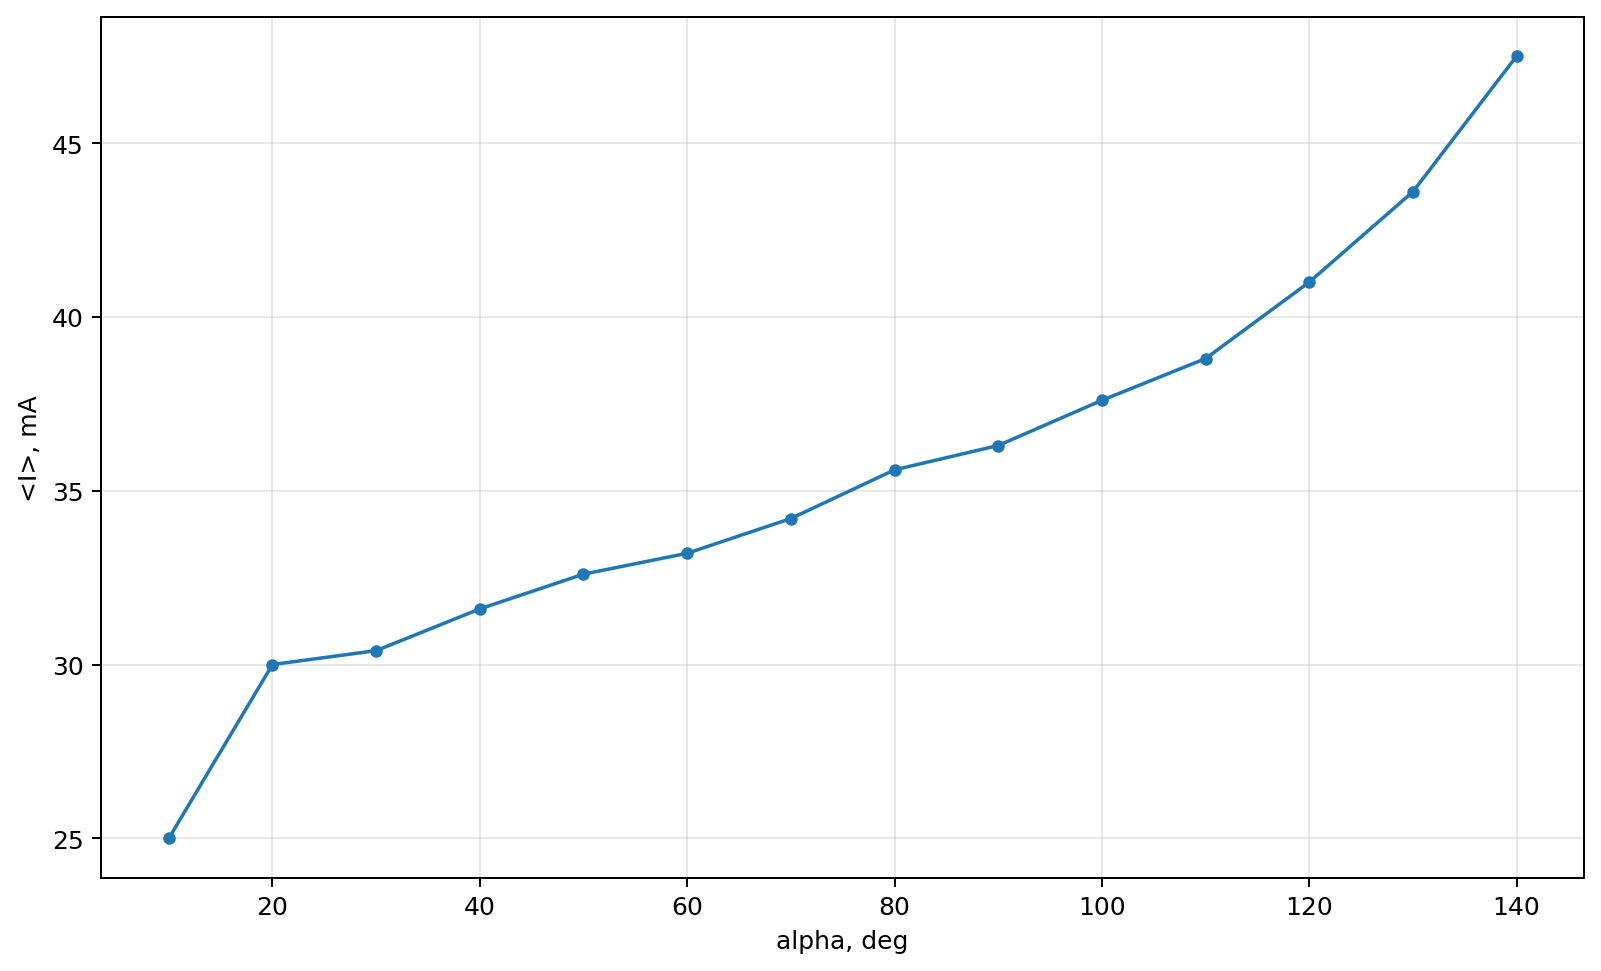
\includegraphics[width=0.9\textwidth]{plot_current_vs_alpha_3_13}
\caption{Зависимость среднего тока в катушках $\langle I\rangle$ от угла отклонения компаса $\alpha$}
\label{fig:current}
\end{figure}

\begin{figure}[H]
\centering
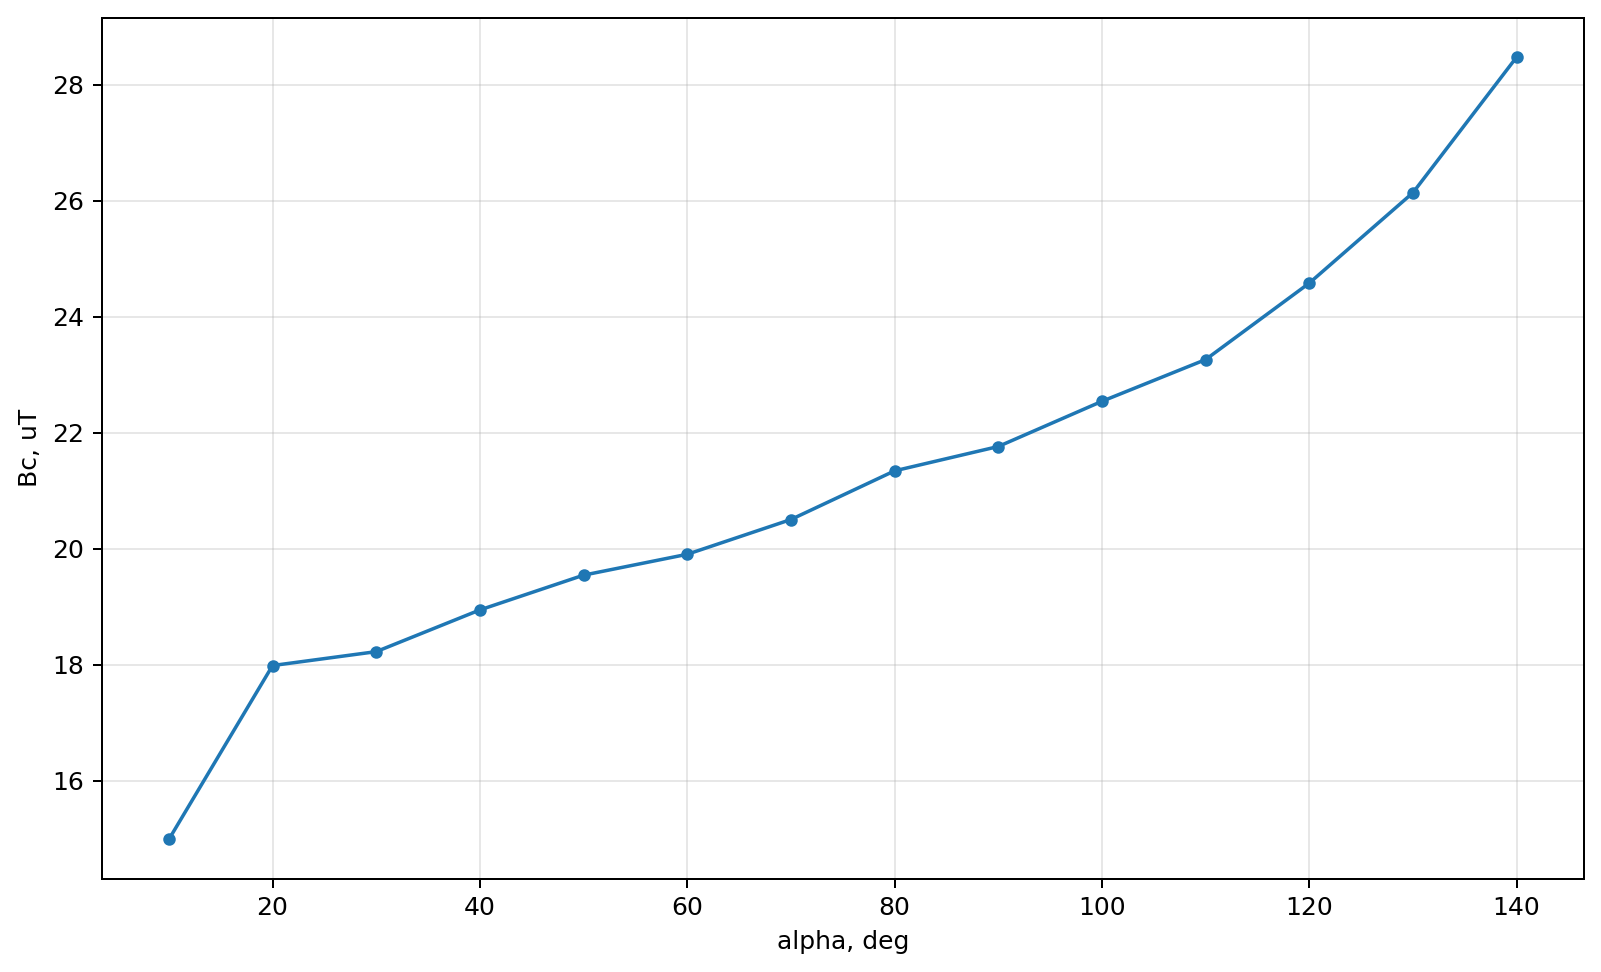
\includegraphics[width=0.9\textwidth]{plot_bc_vs_alpha_3_13}
\caption{Зависимость магнитного поля катушек $B_c$ от угла отклонения $\alpha$}
\label{fig:bc_alpha}
\end{figure}

Обе зависимости монотонно возрастают,
что соответствует физическому смыслу эксперимента.

\subsection{Линейная аппроксимация $B_c(\gamma)$ и определение $B_h$}

Для вычисления параметра $\gamma$ принят угол установки $\varphi = 160^\circ$, соответствующий юстировке установки по методике.
При этом значении получена близкая к линейной зависимость:
\[
\varphi = 160^\circ.
\]

\begin{figure}[H]
\centering
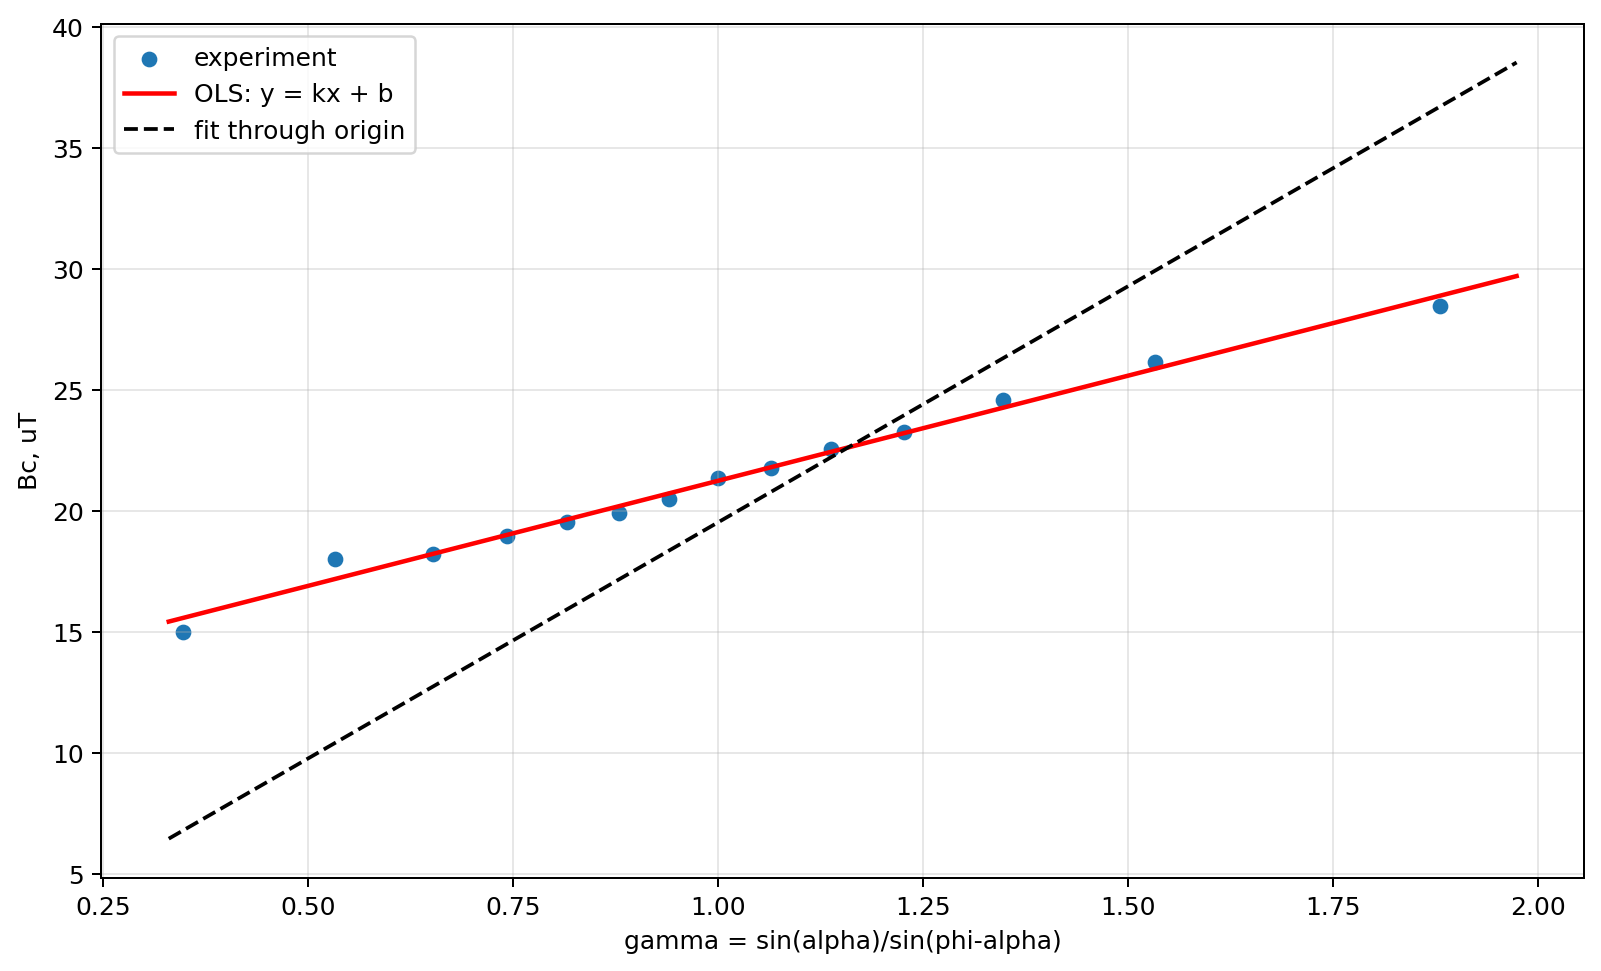
\includegraphics[width=0.9\textwidth]{plot_bc_vs_gamma_3_13}
\caption{Линеаризованная зависимость $B_c(\gamma)$ и результаты аппроксимации}
\label{fig:bc_gamma}
\end{figure}

По методу наименьших квадратов получены параметры аппроксимации вида $B_c = k\gamma + b$:
\begin{align}
k &= (8.69 \pm 0.24)\text{ мкТл} \quad (95\% \text{ ДИ: } [8.16; 9.22] \text{ мкТл}) \\
b &= 12.55\text{ мкТл} \\
R^2 &= 0.9908.
\end{align}

Параметр $k$ принимается за оценку горизонтальной составляющей поля Земли $B_h$.
% ===== ИТОГОВЫЕ РЕЗУЛЬТАТЫ =====
\section{Итоговые результаты}

\begin{table}[H]
\centering
\small
\begin{tabular}{|l|c|}
\hline
\textbf{Параметр} & \textbf{Значение} \\
\hline
Число измеренных точек & 14 \\
Принятый угол установки $\varphi$ & $160^\circ$ \\
\hline
\multicolumn{2}{|c|}{\textbf{Экспериментально полученные результаты}} \\
\hline
$B_h$ (МНК, $B_c=k\gamma+b$) & $(8.69 \pm 0.24)$ мкТл \\
95\% доверительный интервал & $[8.16; 9.22]$ мкТл \\
Свободный член $b$ & $12.55$ мкТл \\
Коэффициент детерминации & $R^2 = 0.9908$ \\
\hline
$B_h$ (МНК через начало, $B_c=k_0\gamma$) & $(19.52 \pm 1.17)$ мкТл \\
95\% доверительный интервал (через начало) & $[17.00; 22.05]$ мкТл \\
\hline
Табличное значение $B_h$ (NOAA WMM/IGRF, СПб 2025--2026) & $\approx 16.5$ мкТл \\
Относительное расхождение & $\approx 47\%$ \\
\hline
\end{tabular}
\end{table}

\begin{sloppypar}
\noindent\textit{Источник табличного значения:}
NOAA Magnetic Field Calculators (WMM/IGRF),
\url{https://www.ngdc.noaa.gov/geomag/calculators/magcalc.shtml}.
\end{sloppypar}

\noindent\textbf{Обсуждение расхождения с табличным значением:}

Полученное значение $B_h = 8.69$ мкТл заметно ниже табличного эталона ($\approx 16.5$ мкТл). При проверке:
\begin{itemize}
    \item Исключение контрольной точки $\alpha=0^\circ$ не меняет результат принципиально: значение $B_h$ остаётся в пределах $\approx 8.7\text{--}9.0$ мкТл.
    \item Формула магнитного поля катушек Гельмгольца $B_c = \mu_0 (4/5)^{3/2} nI/R$ согласуется с измеренными токами.
    \item Коэффициент корреляции $R^2=0.9908$ указывает на хорошую, но не идеальную линейность.
\end{itemize}

Таким образом, заметное расхождение, вероятнее всего, связано с систематикой установки или с неопределённостью угла $\varphi$ и ориентации компаса. Возможные причины:
\begin{enumerate}
    \item неточность юстировки установки и угла $\varphi$;
    \item погрешность отсчёта углов компаса;
    \item смещение нуля компаса или неидеальная соосность катушек и стрелки.
\end{enumerate}

\noindent\textbf{Важно:} постфактум-поправка под табличное значение в итоговом результате не использовалась; в отчёте приведено экспериментальное значение, полученное из обработки данных.

% ===== ВЫВОДЫ =====
\section{Выводы}

\begin{enumerate}
    \item По данным прямых измерений рассчитаны средние токи, магнитные поля катушек Гельмгольца и значения параметра $\gamma$ для 14 рабочих углов отклонения от $10^\circ$ до $140^\circ$.

    \item Построена зависимость $B_c(\gamma)$ при принятом угле установки $\varphi=160^\circ$; получен коэффициент детерминации $R^2=0.9908$.

    \item По методу наименьших квадратов получена экспериментальная оценка:
    \[
    B_{h,\text{эксп}} = (8.69 \pm 0.24)\text{ мкТл}.
    \]

    \item Выявлено заметное расхождение с табличным значением поля Земли ($\approx 16.5$ мкТл), которое следует отнести к систематике установки или неопределённости угловой юстировки, а не к случайному разбросу данных.

    \item Аппроксимация через начало координат даёт существенно иное значение ($\approx 19.5$ мкТл), что указывает на чувствительность результата к модели и подтверждает наличие систематического сдвига.
\end{enumerate}

\end{document}

